\documentclass[10pt]{article}

\usepackage{amsmath}
\usepackage{graphicx}
\usepackage{microtype}
\usepackage{booktabs}
\usepackage{subfigure}
\usepackage{tabularx}
\setlength{\textwidth}{6.5in}
\setlength{\oddsidemargin}{0in}
\setlength{\evensidemargin}{0in}
\setlength{\textheight}{9.0in}
\setlength{\topmargin}{0in}
\setlength{\headheight}{0in}
\setlength{\headsep}{0in}
\setlength{\footskip}{0.333333in}
\usepackage{graphicx}
\usepackage{indentfirst} 


\usepackage[a4paper,left=20mm,right=20mm,top=25mm,bottom=25mm]{geometry}

	\title{
		\textbf{Homework 1 for Advanced Machine Learning}
	}
	\author{Shanghao Shi}

\begin{document}
	\maketitle
	This is the writing part homework of the machine learning class CS5824. This homwork contains two sections, the first one is the answer of question 1 and the second section is the answer for question 2. In order to make my homework more readable, this homework will restate the question before giving out its answer.
	
	\section{Decision tree}
	\subsection{Question}
	Show what the recursive decision tree learning algorithm would choose for the first split of the following dataset:
	
	\begin{center}
	\begin{tabular}{c|cccc|c}
		\toprule
		ID & $X_1$ & $X_2$& $X_3$ & $X_4$ & $Y$\\
		\midrule
		1 & 0 & 0 & 0 & 0 & 0\\
		2 & 0 & 0 & 0 & 1 & 0\\
		3 & 0 & 0 & 1 & 0 & 0\\
		4 & 0 & 0 & 1 & 1 & 0\\
		5 & 0 & 1 & 0 & 0 & 0\\
		6 & 0 & 1 & 0 & 1 & 1\\ 
		7 & 0 & 1 & 1 & 0 & 1\\ 
		8 & 0 & 1 & 1 & 1 & 1\\ 
		9 & 1 & 0 & 0 & 0 & 1\\ 
		10 & 1 & 0 & 0 & 1 & 1\\ 
		\bottomrule
	\end{tabular}
	\end{center}

	Assume that the criterion for deciding the best split is entropy reduction (i.e., information gain). If there are any ties, choose the first feature to split on tied for the best score. Show your calculations in your response.
	
	\subsection{Answer}
	First we will calculate the entrophy of the whole dataset $\cal D$. There are 5 samples having the $Y$ values 1 and another 5 samples having $Y$ values 0. Thus the entrophy of the whole dataset $\cal D$ is:
	\begin{flalign}
		H(D)=\sum_{i=1}^{2} -p_i log(p_i)=0.5log(2)+0.5log(2)=1 bit
	\end{flalign}\par
	Then we choose feature $X_1$ to be the first decision rule. We will see the information gain of this feature. Using this rule, we divide the dataset $\cal D$ into two dataset ${\cal D}_1$ and ${\cal D}_2$. The information gain is:
	\begin{equation}
	\begin{aligned}
	infoGain(X_1)&=H({\cal D})-\{\frac{\vert {\cal D}_1\vert}{\vert \cal D\vert}H({\cal D}_2)+\frac{\vert {\cal D}_2\vert}{\vert \cal D\vert}H({\cal D}_2)\}\\
	&=1-\frac{8}{10}\{ \frac{5}{8}log(\frac{8}{5})+\frac{3}{8}log(\frac{8}{3})\}=0.2365 bit
	\end{aligned}
	\end{equation}  
	
	Using the same method, we then calculate the information gain of feature $X_2$, $X_3$, $X_4$:
	\begin{equation}
	\begin{aligned}
	infoGain(X_2)&=H({\cal D})-\{\frac{\vert {\cal D}_1\vert}{\vert \cal D\vert}H({\cal D}_2)+\frac{\vert {\cal D}_2\vert}{\vert \cal D\vert}H({\cal D}_2)\}\\
	&=1-\frac{6}{10}\{ \frac{4}{6}log(\frac{6}{4})+\frac{2}{6}log(\frac{6}{2})\}-\frac{4}{10}\{ \frac{1}{4}log(\frac{4}{1})+\frac{3}{4}log(\frac{4}{3})\}=0.1245 bit
	\end{aligned}
	\end{equation} 

	\begin{equation}
	\begin{aligned}
	infoGain(X_3)&=H({\cal D})-\{\frac{\vert {\cal D}_1\vert}{\vert \cal D\vert}H({\cal D}_2)+\frac{\vert {\cal D}_2\vert}{\vert \cal D\vert}H({\cal D}_2)\}\\
	&=1-\frac{6}{10}\{ \frac{2}{4}log(\frac{4}{2})+\frac{2}{4}log(\frac{4}{2})\}-\frac{4}{10}\{ \frac{3}{6}log(\frac{6}{3})+\frac{3}{6}log(\frac{6}{3})\}=0 bit
	\end{aligned}
	\end{equation} 

	\begin{equation}
	\begin{aligned}
	infoGain(X_4)&=H({\cal D})-\{\frac{\vert {\cal D}_1\vert}{\vert \cal D\vert}H({\cal D}_2)+\frac{\vert {\cal D}_2\vert}{\vert \cal D\vert}H({\cal D}_2)\}\\
	&=1-\frac{5}{10}\{ \frac{2}{5}log(\frac{5}{2})+\frac{3}{5}log(\frac{5}{3})\}-\frac{5}{10}\{ \frac{2}{5}log(\frac{5}{2})+\frac{3}{5}log(\frac{5}{3})\}=0.0290 bit
	\end{aligned}
	\end{equation} \par
	Compare the four information gains we get above, we find that $X_1$ is the best decision rule.
	\par
	
	Then we come to see dataset ${\cal D}_1$ and dataset ${\cal D}_2$. All data in ${\cal D}_2$ are in the same class, so we just need to consider ${\cal D}_1$. There are 8 examples in ${\cal D}_1$. 5 of them belong to class 0 and 3 of them belong to class 1. So the entrophy of ${\cal D}_1$ is:
	\begin{equation}
		H(D_1)=\sum_{i=1}^{2} -p_i log(p_i)=\frac{5}{8}log(\frac{8}{5})+\frac{3}{8}log(\frac{8}{3})=0.9544 bit
	\end{equation}
	
	We will also choose another best decision rule for ${\cal D}_1$. This rule will divide ${\cal D}_1$ to two dataset ${\cal D}_3$ and ${\cal D}_4$. Calculate the information gain of $X_2$, $X_3$, $X_4$ to get this decision.
	
	\begin{equation}
	\begin{aligned}
	infoGain(X_2)&=H({\cal D}_1)-\{\frac{\vert {\cal D}_3\vert}{\vert {\cal D}_1 \vert}H({\cal D}_3)+\frac{\vert {\cal D}_4\vert}{\vert {\cal D}_1 \vert}H({\cal D}_4)\}\\
	&=0.9544-\frac{4}{8}\{ \frac{1}{4}log(\frac{4}{1})+\frac{3}{4}log(\frac{4}{3})\}=0.5488 bit
	\end{aligned}
	\end{equation} 
	
	\begin{equation}
	\begin{aligned}
	infoGain(X_3)&=H({\cal D}_1)-\{\frac{\vert {\cal D}_3\vert}{\vert {\cal D}_1 \vert}H({\cal D}_3)+\frac{\vert {\cal D}_4\vert}{\vert {\cal D}_1 \vert}H({\cal D}_4)\}\\
	&=0.9544-\frac{4}{8}\{ \frac{1}{4}log(\frac{4}{1})+\frac{3}{4}log(\frac{4}{3})\}-\frac{4}{8}\{ \frac{2}{4}log(\frac{4}{2})+\frac{2}{4}log(\frac{4}{2})\}=0.0488 bit
	\end{aligned}
	\end{equation} 
	
	\begin{equation}
	\begin{aligned}
	infoGain(X_4)&=H({\cal D}_1)-\{\frac{\vert {\cal D}_3\vert}{\vert {\cal D}_1 \vert}H({\cal D}_3)+\frac{\vert {\cal D}_4\vert}{\vert {\cal D}_1 \vert}H({\cal D}_4)\}\\
	&=0.9544-\frac{4}{8}\{ \frac{1}{4}log(\frac{4}{1})+\frac{3}{4}log(\frac{4}{3})\}-\frac{4}{8}\{ \frac{2}{4}log(\frac{4}{2})+\frac{2}{4}log(\frac{4}{2})\}=0.0488 bit
	\end{aligned}
	\end{equation} 
	\par
    From the result we can see that feature $X_2$ is the second best decision rule. This rule will divide the dataset into Two different parts ${\cal D}_3$ and ${\cal D}_4$. Both ${\cal D}_3$ and ${\cal D}_4$ contain 4 examples. All exmples in ${\cal D}_4$ are in the same class and we do not have to consider it. But in ${\cal D}_3$, 3 examples belong to class 1 and 1 example belongs to class 0. Therefore we can get that the entrophy of this dataset is: 
    \begin{equation}
    H(D_3)=\sum_{i=1}^{2} -p_i log(p_i)=\frac{1}{4}log(\frac{4}{1})+\frac{3}{4}log(\frac{4}{3})=0.8113 bit
    \end{equation}\par
    Using the same method we calculte the information gain of each feature. Using these features, dataset ${\cal D}_3$ is divided to two dataset ${\cal D}_5$ and ${\cal D}_6$.
    \begin{equation}
    \begin{aligned}
    infoGain(X_3)&=H({\cal D}_3)-\{\frac{\vert {\cal D}_5\vert}{\vert {\cal D}_3\vert}H({\cal D}_5)+\frac{\vert {\cal D}_6\vert}{\vert {\cal D}_3\vert}H({\cal D}_6)\}\\
    &=0.8113-\frac{2}{4}\{ \frac{1}{2}log(\frac{2}{1})+\frac{1}{2}log(\frac{2}{1})\}=0.3113 bit
    \end{aligned}
    \end{equation} 
    
    \begin{equation}
    \begin{aligned}
    infoGain(X_4)&=H({\cal D}_3)-\{\frac{\vert {\cal D}_5\vert}{\vert {\cal D}_3\vert}H({\cal D}_5)+\frac{\vert {\cal D}_6\vert}{\vert {\cal D}_3\vert}H({\cal D}_6)\}\\
    &=0.8113-\frac{2}{4}\{ \frac{1}{2}log(\frac{2}{1})+\frac{1}{2}log(\frac{2}{1})\}=0.3113 bit
    \end{aligned}
    \end{equation} \par
	Two information gain are the same and we choose this first feature $X_3$ as our best decision rule.\par
	Finally, we will chose $X_4$ as the last decision rule. Having all of our decstion rules, we can get our decision tree and it is shown in the following picture.\\
	\begin{figure}
		\begin{center}
		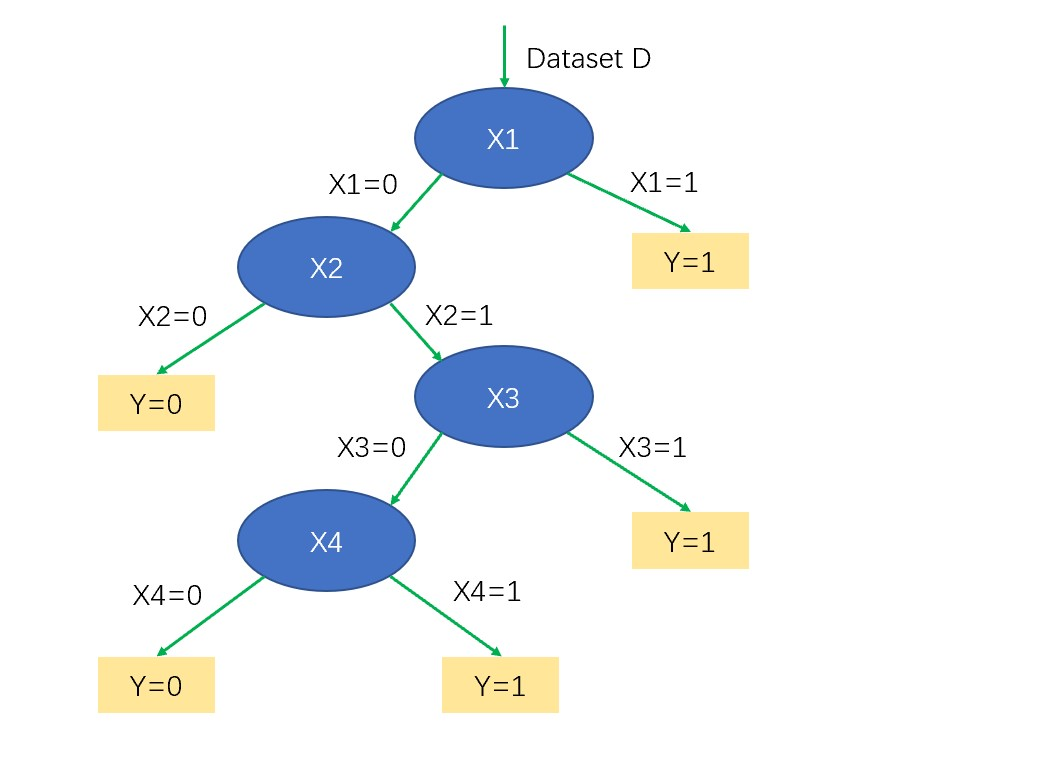
\includegraphics[scale=0.65]{decision_tree.jpg}
		\caption{Decision Tree}
		\end{center}
	\end{figure}
	
	
	
	
			
	
	\section{Bayes analysis}
	\subsection{Question}
	A Bernoulli distribution has the following likelihood function for a data set $\cal D$:
	\begin{align}
	p({\cal D} | \theta) &= \theta^{N_1} (1 - \theta)^{N_0},
	\label{eq:bernoulli}
	\end{align}\\
	where $N_1$ is the number of instances in data set $\cal D$ that have value 1 and $N_0$ is the number in $\cal D$ that have value 0. The maximum likelihood estimate is 
	\begin{align}
	\hat{\theta} &= \frac{N_1}{N_1 + N_0}.
	\label{eq:mle}
	\end{align}
	
	\begin{enumerate}
		
		\item Derive the maximum likelihood estimate above by solving for the maximum of the likelihood.
		
		\item Suppose we now want to maximize a posterior likelihood
		\begin{align}
		p(\theta | {\cal D}) &= \frac{p({\cal D} | \theta) p(\theta)}{p({\cal D})},
		\end{align}
		where we use the Bernoulli likelihood and a (slight variant\footnote{For convenience, we are using the exponent of $\alpha$ instead of the standard $\alpha-1$.} of a) symmetric Beta prior over the Bernoulli parameter
		\begin{align}
		p(\theta) &\propto \theta^{\alpha} (1 - \theta)^{\alpha}.
		\end{align}
		Derive the maximum posterior mean estimate.
		
	\end{enumerate}



	\subsection{Answer}
	\subsubsection{1}
		The maximum likelihood estimate of $\theta$ is the value that maximizing likelihood function. We have know that the likelihood function is $p({\cal D} | \theta) = \theta^{N_1} (1-\theta)^{N_0}$. Thus we will derive on likelihood function to find its extremum.
		
		\begin{equation}
		\begin{aligned}
			\frac{\mathrm{d}p({\cal D} | \theta)}{\mathrm{d}\theta}&=N_1 \theta^{N_1-1}(1-\theta)^{N_0}-N_0 \theta^{N_1} (1-\theta)^{N_0-1} \\
			&=N_1 (1-\theta \frac{N_1+N_0}{N_1})\theta^{N_1-1}(1-\theta)^{N_0-1}
		\end{aligned}
		\end{equation}
		\par
		From the equation above, we can see that when $\theta=0, 1, \frac{N_1}{N_1+N_0}$, $p'({\cal D} | \theta)$ has the value of zero.\par
		Further, we can also find that when $0<\theta<\frac{N_1}{N_1+N_0}$, the derivative funtion of likelihood function $p'({\cal D} | \theta)$ is strictly positive and when $\frac{N_1}{N_1+N_0}<\theta<1$, the derivative funtion of likelihood function $p'({\cal D} | \theta)$ is strictly negative. Thus we get that likelihood function reaches its maximum at point $\theta=\frac{N_1}{N_1+N_0}$. 
		Therefore, the maximum likelihood estimate of $\theta$ is $\hat{\theta}=\frac{N_1}{N_1+N_0}$.
		 
		
	
	
	
	\subsubsection{2}
	As $p(\cal D)$ will not change when dataset $\cal D$ is fixed, the value of $\theta$ that maximum posterior likelihood $p(\theta|\cal D)$ is the same with the value that maximum $p({\cal D} |\theta) p(\theta)$. Thus we will only consider $p({\cal D} |\theta)p(\theta)$ instead of $p(\theta|{\cal D})$. We will derive $p({\cal D} |\theta)p(\theta)$ to see the result.
	
	\begin{equation}
	\begin{aligned}
	\frac{\mathrm{d}p({\cal D} | \theta)p(\theta)}{\mathrm{d}\theta}&=\frac{\mathrm{d}\theta^{N_1+\alpha}(1-\theta)^{N_0+\alpha}}{\mathrm{d}\theta}\\
	&=(\alpha+ N_1) \theta^{N_1+\alpha-1}(1-\theta)^{N_0}-(\alpha+ N_0) \theta^{N_1+\alpha} (1-\theta)^{N_0+\alpha-1} \\
	&=(N_1+\alpha) (1-\theta \frac{N_1+N_0+2 \alpha}{N_1+\alpha})\theta^{N_1-1}(1-\theta)^{N_0-1}
	\end{aligned}
	\end{equation}\\
	\par
	From the equation above we can get that when $\theta=0, 1$ and  $\frac{N_1+\alpha}{N_1+N_0+2 \alpha}$, $\frac{\mathrm{d}p({\cal D} | \theta)p(\theta)}{\mathrm{d}\theta}=0$.So only at these points can the function get its extremum. 
	
	\par
	
	When $0<\theta<\frac{N_1+\alpha}{N_1+N_0+2 \alpha}$, $\frac{\mathrm{d}p({\cal D} | \theta)p(\theta)}{\mathrm{d}\theta}$ is strictly positive and function is monotone increasing. When $\frac{N_1+\alpha}{N_1+N_0+2 \alpha}<\theta<1$, $\frac{\mathrm{d}p({\cal D} | \theta)p(\theta)}{\mathrm{d}\theta}$ is strictly negative and the function is monotone decreasing. Thus the function get its maximum at the point $\theta=\frac{N_1+\alpha}{N_1+N_0+2 \alpha}$. So the maximum posterior estimate of parameter $\theta$ is $\hat{\theta}=\frac{N_1+\alpha}{N_1+N_0+2 \alpha}$.		
		
			
\end{document}